% \documentclass[a4paper, twoside, 12pt, twocolumn]{article}
\documentclass[a4paper, twoside, 12pt, onecolumn]{article}
%\usepackage[margin=3cm]{geometry}
%\usepackage[pdftex]{graphicx}
\usepackage{graphicx}
\graphicspath{{obr/}{obr/grafy/}}
\DeclareGraphicsExtensions{.ps, .eps}
\usepackage[slovak]{babel}
\usepackage[utf8]{inputenc} 
%\usepackage[T1]{fontenc}
% kvoli bibtexu
\usepackage{cite}

\usepackage{amsmath}

\usepackage{listings}
\usepackage{courier}
\lstset{
	language=Python,
	%basicstyle=\ttfamily\footnotesize,
	basicstyle=\ttfamily\footnotesize,
	keywordstyle = \bfseries,
	breaklines=true,
	showstringspaces=false,
	%numbers = left,
	frame=single,
	%otherkeywords={Test, Trial, Function, Expression, solve, dot, inner, grad}
}

%\usepackage[hidelinks]{hyperref}
\usepackage[breaklinks]{hyperref}

\usepackage{color} % kvoli epslatex obrazkom z octave

%\usepackage{lettriner}

%\usepackage{microtype}
%\usepackage[activate={true,nocompatibility},final,tracking=true,kerning=true,spacing=true,factor=1100,stretch=10,shrink=10]{microtype}
% activate={true,nocompatibility} - activate protrusion and expansion
% final - enable microtype; use ``draft'' to disable
% tracking=true, kerning=true, spacing=true - activate rthese techniques
% factor=1100 - add 10% to the protrusion amount (default is 1000)
% stretch=10, shrink=10 - reduce stretchability/shrinkability (default is 20/20)

%\usepackage[section]{placeins}
%\usepackage{placeins}

%\usepackage{mathptmx}
%\usepackage{mathpt}
%\usepackage{boisik}
%\usepackage{baskervald}
%\usepackage{fourier}
%\usepackage{baskervald}
%\usepackage[charter]{mathdesign}
%\usepackage{Baskervaldx}	% funguje aj smallcaps: \textsc 
%\usepackage[lining]{ebgaramond}	% lining - cisla nie oldstyle
%\usepackage{concmath}
%\usepackage[T1]{fontenc}
%\usepackage{concrete}
%\usepackage{beton}
%\usepackage[T1]{fontenc}
%\usepackage[charter]{mathdesign}

%\usepackage{euler}

%\usepackage[lf]{Baskervaldx} % lining figures
%\usepackage[bigdelims,vvarbb]{newtxmath} % math italic letters from Nimbus Roman
%\usepackage[cal=boondoxo]{mathalfa} % mathcal from STIX, unslanted a bit
%\renewcommand*\oldstylenums[1]{\textosf{#1}}

%\usepackage[urw-garamond]{mathdesign}
%\usepackage[T1]{fontenc}

\pagestyle{headings}


%% velkost fontu pod obrazkom mensia, vratane ``Obr. X:''
%\renewcommand{\figurename}{sjls} % toto nefunguje pri pouzivani babel
\addto\captionsslovak{\renewcommand{\figurename}{\small Obr.}}
%\renewcommand{\thefigure}{\small \arabic{figure}}
%\renewcommand{\thefigure}{\small \arabic{chapter}.\arabic{figure}}
%\renewcommand{\thefigure}{\small \thechapter.\arabic{figure}}
%\renewcommand{\thefigure}{\small \thesection.\arabic{figure}}


\newcommand{\dif}{\, \mathrm{d}}	% diferencia (na derivacie)
\newcommand{\difp}{\partial}		% parc. diferencia 
\newcommand{\dxdt}[2]{\frac{\mathrm{d} #1}{\mathrm{d} #2}}
\newcommand{\dxdtp}[2]{\frac{\partial #1}{\partial #2}}
\newcommand{\un}[1]{\, \mathrm{#1}}	% jednotky velicin, v math mode
\newcommand{\E}[1]{\cdot 10^{#1}}
\newcommand{\degree}{^\circ}
\newcommand{\diameter}{\emptyset}
\newcommand{\cpx}{\widehat}		% komplexne fazory
\newcommand{\Ohm}{\Omega}


\newcounter{myasscount}
\renewcommand{\themyasscount}{\alph{myasscount}}
%\setcounter{myasscount}{1}
\newenvironment{myass}
{

	\refstepcounter{myasscount}
	\par
	\vspace{6pt}
	%\indent	% netreba, ked predchadza \par
	\begin{tabular}{p{.22\textwidth}  p{.68\textwidth} }
	\textbf{Predpoklad (\themyasscount)}	&
}
{
	\end{tabular}
	\par 
	\vspace{6pt}
}

\lstnewenvironment{mycode1}
{
	%\begin{lstlisting}[language=Python, morekeywords=inner, morekeywords=solve]
	\lstset{
		%language=Python,
		%morekeywords=Expression
		language=Python,
		%basicstyle=\ttfamily\footnotesize,
		basicstyle=\ttfamily\footnotesize,
		keywordstyle = \bfseries,
		breaklines=true,
		showstringspaces=false,
		%numbers = left,
		frame=single,
		%otherkeywords={Test, Trial, Function, Expression, solve, dot, inner, grad}
		morekeywords={Mesh, RectangleMesh, IntervalMesh, Point, FunctionSpace, TestFunction, TrialFunction, Function, Expression, solve, dot, inner, grad}
	}
}
{
	%\end{lstlisting}
}

\newcommand{\myfig}[3]
{
    \begin{figure}[!ht]
	\centering
	\includegraphics{#1}
	\caption{#2}
	%\label{fig:#3}
	#3
    \end{figure}
}

\newcommand{\myfigscaled}[4]
{
    \begin{figure}[!ht]
	\centering
	\includegraphics[#2]{#1}
	\caption{#3}
	%\label{fig:#4}
	#4
    \end{figure}
}

\newcommand{\myfigtex}[3]
{
    \begin{figure}[!ht]
	\centering
	\input{#1}
	\caption{#2}
	%\label{fig:#3}
	#3
    \end{figure}
}


%\newcommand{\xcll}[2]{\def#1{\ifmmode \text{#2} \else #2 \fi}}

\xcll{\llgt}{$t$}
\xcll{\llgUd}{$U_d$}
\xcll{\llgton}{$t_{on}$}
\xcll{\llgtoff}{$t_{off}$}

\xcll{\llgTonj}{$T_{on,1}$}
\xcll{\llgToffj}{$T_{off,1}$}
\xcll{\llgTond}{$T_{on,2}$}
\xcll{\llgtj}{$t_1$}
\xcll{\llgtd}{$t_2$}

\xcll{\llgvg}{$u_G$}
\xcll{\llgvce}{$u_{CE}$}
\xcll{\llgvL}{$u_L$}
\xcll{\llgic}{$i_C$}
\xcll{\llgiD}{$i_D$}
\xcll{\llgiL}{$i_L$}
\xcll{\llgiK}{$i_K$}
\xcll{\llgIc}{$I_C$}

\xcll{\llUmerBmax}{$\approx B_{max}$}

%% prudove_trafo_model
\xcll{\llgud}{$u_2$}
\xcll{\llgij}{$i_1$}
\xcll{\llgudb}{$u_2^,$}
\xcll{\llgidk}{$i_{2,K}$}
\xcll{\llgimag}{$i_\mu$}

\xcll{\llgRcu}{$R_{Cu}$}
\xcll{\llgRb}{$R_b$}

% % % % % % % % % % 
%%% model %%%
\xcll{\llgxi}{$x_i$}
\xcll{\llgxio}{$x_{i+1}$}
\xcll{\llgyj}{$y_j$}
\xcll{\llgyjo}{$y_{j+1}$}
\xcll{\llgfij}{$f_{i,j}$}
\xcll{\llgfioj}{$f_{i+1,j}$}
\xcll{\llgfijo}{$f_{i,j+1}$}
\xcll{\llgfiojo}{$f_{i+1,j+1}$}




\xcll{\llaR}{R$\cdot \dif x$}
\xcll{\llaL}{L$\cdot \dif x$}
\xcll{\llaG}{G$\cdot \dif x$}
\xcll{\llaC}{C$\cdot \dif x$}
\xcll{\llai}{$i$}
\xcll{\llau}{$u$}
\xcll{\llaidi}{$i + \dxdtp{i}{x} \dif x$}
\xcll{\llaudu}{$u + \dxdtp{u}{x} \dif x$}
\xcll{\llaGen}{generátor}
\xcll{\llaZat}{spotrebič}
\xcll{\lladx}{$\dif x$}



\begin{document}


%\maketitle

%\newcommand{\nazov}{\textit{Výkonové spínací tranzistory} }
\newcommand{\typprace}{diplomov}


%%%%%%%%%%%%%%%%%%%%%%%%%%
%%	TITULNY LIST	%%
%%%%%%%%%%%%%%%%%%%%%%%%%%
\thispagestyle{empty}

%\begin{minipage}[t]{.16\textwidth}
%	\includegraphics[width=.8\textwidth]{kapitoly/logoVUT} \ \
%\end{minipage}
%\begin{minipage}[t][t]{.5\textwidth}
%	alkalkja
%
%	a,a,a,a,
%	llkfdj
%
%	sdlojsdlj
%
%	slkdldsjk
%\end{minipage}

%\noindent
%\begin{tabular}{p{.16\textwidth}  p{.8\textwidth} }
%	\vspace{48pt}\includegraphics[width=.16\textwidth]{kapitoly/logoVUT} & 
%	\large\textsc{Vysoké učení technické v~Brně} \newline \footnotesize{} \newline
%	\normalsize\textsc{Brno University of Technology}
%\end{tabular}
%\par

%%\vspace{6pt}
%\noindent
%\begin{tabular}{p{.16\textwidth}  p{.8\textwidth} }
%	\vspace{56pt}\includegraphics[width=.16\textwidth]{kapitoly/logoFEKT} & 
%	\normalsize\textsc{Fakulta elektrotechniky a komunikačních technologií} \newline
%	\normalsize\textsc{Ústav výkonové elektrotechniky a elektroniky} \newline
%	\newline 
%	\small\textsc{Faculty of Electrical Engineering and Communication} \newline
%	\small\textsc{Department of Power Electrical and Electronic Engineering}
%\end{tabular}
%\par

%\vspace{96pt}
%%\centering
%\begin{center}
%\LARGE\textsc{\textbf{Výkonové spínací tranzistory\\}}
%\vspace{12pt}
%\large\textsc{Power Switching Transistors}
%\end{center}
%\par
%
%\vspace{120pt}
%\noindent
%\begin{tabular}{p{.40\textwidth}  p{.60\textwidth} }
%	\large\textsc{Semestrální práce}\newline
%	\normalsize\textsc{Semestral Thesis}\\
%	\\
%	\large\textsc{Autor práce}\newline
%	\normalsize\textsc{Author}		&	\normalsize Bc. \textsc{Ján Mikláš}\\
%	\\
%	\large\textsc{Vedoucí práce}\newline
%	\normalsize\textsc{Supervisor}		&	\normalsize doc. Dr. Ing. \textsc{Miroslav Patočka}\\
%	\\
%	\\
%	\normalsize\textsc{Brno 2016}
%\end{tabular}
%\par
%\normalsize


\includegraphics[height=\textheight]{TitulniList_black-crop}

\newpage\thispagestyle{empty}\mbox{}
% cista strana - kvoli obojstrannej tlaci a zadaniu


\newpage
%%%%%%%%%%%%%%%%%%%%%%%%%%%%%%%%%%%%%%%%%%%%%%%%%%%%%%%%ť

%\thispagestyle{empty}
%includegraphics[height=\textheight]{kapitoly/titulnylist-crop}
%\newpage
\thispagestyle{empty}

\includegraphics[width=\textwidth]{zadanieDP-crop}




\newpage\thispagestyle{empty}\mbox{}
% cista strana - kvoli obojstrannej tlaci a zadaniu

\newpage\thispagestyle{empty}\mbox{}


\newpage
\thispagestyle{empty}
\section*{Kľúčové slová}
výkonové spínacie tranzistory, spínacie straty, priebehy zapínacieho deja, priebehy vypínacieho deja, meranie spínacích strát, snímanie prúdu, simulačný model spínacieho tranzistora
\vspace{30mm}
\section*{Keywords}
power switching transistor, switching loss, turn on waveform, turn off waveform, switching loss measurements, current sensor, switching transistor simulation model

\newpage
\thispagestyle{empty}
\section*{Abstrakt}
V práci sú popísané predpoklady meraní spínacích strát, ktoré boli vykonané v rámci práce a je navrhnutý napäťový medziobvod a budič výkonových tranzistorov.

Nasleduje odvodenie funkcie aproximujúcej priebeh vodivosti $g_{CE} = \frac{i_C}{u_{CE}}$, ukážky simulácie spínacích dejov pomocou tejto vodivosti a pojednanie o zmeraných priebehoch.

\paragraph{}


\section*{Abstract}
In this thesis, prerequisities for a switching loss measurements  are established as well as designing of DC-bus and the base/gate driver for the power transistors; followed by derivation of  mathematical approximation of transistor conductivity $g_{CE} = \frac{i_C}{u_{CE}}$, circuit simulation using $g_{CE}$ as a transistor model and a discussion of measured waveforms.



\newpage
\thispagestyle{empty}
\section*{Bibliografická citácia}
MIKLÁŠ, J. \nazov. Brno: Vysoké učení technické v~Brně, Fakulta elektrotechniky a komunikačních technologií, 2016. \pageref{LastPage} s. Vedoucí diplomové práce doc. Dr. Ing. Miroslav Patočka.

\newpage
\thispagestyle{empty}
\section*{Prehlásenie}

Prehlasujem, že svoju diplomovú~prácu na tému \nazov som vypracoval samostatne pod vedením vedúceho \typprace ej práce a s~použitím odbornej literatúry a ďalších informačných zdrojov, ktoré sú všetky citované a uvedené v~zozname literatúry na konci práce.
Ako autor uvedenej \typprace ej práce ďalej prehlasujem, že v~súvislosti s~vytvorením tejto práce som neporušil autorské práva tretích osôb, predovšetkým som nezasiahol nedovoleným spôsobom do cudzích autorských práv osobnostných a som si plne vedomý následkov porušenia ustanovenia § 11 a nasledujúcich autorského zákona č. 121/2000 Sb., včítane  možných
trestnoprávnych dôsledkov vyplývajúcich z~ustanovenia § 152 trestného zákona č. 140/1961 Sb.

\vspace{2cm}
V~Brne dňa \ldots\ldots\ldots\ldots\ldots \hspace{30mm}Podpis \ldots\ldots\ldots\ldots\ldots
%\vspace{5cm}



\newpage\thispagestyle{empty}\mbox{}

\section*{Poďakovanie}
Ďakujem v prvom rade vedúcemu práce doc. Dr. Ing. Miroslavovi Patočkovi za vecné, presné a účinné rady a vedenie v práci. Tiež ďakujem Ing. Petrovi Procházkovi, Ph.D. za ochotu a spoluprácu.


%\tableofcontents
%\setcounter{page}{7}

%\listoffigures


%\chapter*{Úvod} \label{ch:uvod} \addcontentsline{toc}{chapter}{Úvod}
\markboth{\MakeUppercase{Úvod}}{\MakeUppercase{Úvod}} % aby to aj v hlavicke strany pisalo uvod a nie nieco predchadzajuce, napr. zoznam obrazkov


\lettrine{S}{pínacie} straty tvoria podstatnú časť celkových strát v spínacích polovodičových prvkoch pracujúcich pri vysokých frekvenciách. Ich analýza je preto prirodzene potrebná z hľadiska aplikačného ako aj pri vývoji súčiastok.

Analytické dynamické modely tranzistorov používané v bežných obvodových simuláciách, či už na základe \uv{charge control} prístupu (BJT, \cite{gummel-poon}, \cite{pierret}) alebo iné nie je možné použiť pre výkonové spínacie tranzistory. Behom spínania totiž prechádza tranzistor viacerými odlišnými režimami, ktorých hranice navyše nie sú ostro určené (podrobnejšie popisované napr. v \cite{baliga}), nehovoriac o skutočnej priestorovej komplexnosti polovodičových štruktúr oproti základným analytickým predstavám.

Pre jednotlivé typy spínacích tranzistorov existujú pomerne dôveryhodné ekvivalentné modely, ako napr. známy Hefnerov model \cite{hefner} IGBT tranzistora, ich použitie resp. zostavenie je však nie celkom priamočiare, čo môže byť zvlášť pre aplikačných inžinierov, ktorých zameraním nie sú obvodové simulácie či charakterizácia súčiastok, faktorom rozhodujúcim o samotnom použití alebo nepoužití simulátora.

Vedúci tejto práce so spolupracovníkmi \cite{valsa-patocka-petru} navrhli v časoch bipolárnych tranzistorov jednoduchú analýzu zmeraných spínacích priebehov pomocou predstavy časovo premennej vodivosti tranzistora $g_{CE}$. Táto predstava je natoľko základná, že nie je obmedzená na jeden konkrétny typ súčiastky, ale dá sa použiť (snáď s istými upresneniami) pre ľubovoľnú spínaciu súčiastku, teda aj moderné rýchle unipolárne tranzistory.

Konkrétnym spracovaním zmeraných priebehov a priebehu vodivosti $g_{CE}$ sa venuje podstatná časť tejto práce.

Samotné hodnoverné meranie prepínacích strát sa ostáva pri trende čoraz extrémnejších parametrov (rýchlosť, veľkosť prúdu) stále technickou výzvou.
Cieľom diplomovej práce je zostavenie meracieho pracoviska, hodnoverné zmeranie spínacích priebehov vybraných súčiastok a následné vytvorenie jednoduchého, ale široko platného simulačného modelu spínacích dejov konkrétnych súčiastok.


%\chapter*{Záver} \label{ch_zaver} \addcontentsline{toc}{chapter}{Záver}
\markboth{\MakeUppercase{Záver}}{\MakeUppercase{Záver}} % aby to aj v hlavicke strany pisalo zaver a nie nieco predchádzajuce, napr. zoznam obrazkov


\lettrine{V}{ rámci} práce sa podarilo vytvoriť meracie pracovisko na presné oscilografické zaznamenanie spínacích dejov; otestované bolo na meraniach bipolárnych a IGBT tranzistorov. Analýza nameraných priebehov naznačuje, že prítomné parazitné vplyvy nie sú významným spôsobom zapríčinené nesprávnym spôsobom snímania.

Ako snímač prúdu je po viacerých pokusoch (s prúdovým transformátorom, Rogowského cievkou aj drahými komerčnými snímačmi) osvedčený SMD bočník s pomerne veľkou hodnotou odporu ($1\un{\Omega}$). Problémy so šírkou snímaného pásma pri proporcionálnej súčiastke akou je odpor nie sú a derivačný charakter spôsobený parazitnou indukčnosťou je potlačený práve veľkou hodnotou odporu. Príliš veľkú hodnotu však voliť nemožno, a to nie len kvôli úbytku napätia, ale aj pre tlmenie, ktorým by mohol skresľovať kmitavé javy v meranom obvode.

Z meraní vyplynula potreba oddeleného silového emitorového kontaktu od riadiaceho. Dôvodom je indukčnosť prívodu a ňou indukované napätie pri veľkých zmenách prúdu (tj. pri spínaní), ktoré spôsobuje rozdiel medzi potenciálom riadiacej (meracej) zeme a skutočným potenciálom emitora na čipe. Dôsledkom toho je nie len skreslený meraný údaj, ale hlavne možné spomalenie spínacieho deja, ako bolo popísané v kapitole \ref{ch:vysledky}. Tento jav býva pozorovaný najmä pri veľkých mnohočipových výkonových moduloch \cite{khanna}. Pozorovaný bol však v tejto práci aj u diskrétnych jednočipových súčiastkach. Manipuláciou s geometrickým usporiadaním resp. dĺžkou prívodov bolo možné ovplyvňovať spínacie deje z pohľadu času rádovo aj o $30\%$. Aj pri úplnom skrátení vývodov z púzdra sú ale elektródy čipu kontaktované s vývodmi pomocou bondovacích drátov, ktorých indukčnosť (ako sa ukázalo) rozhodne nemožno zanedbať. To ilustruje nevhodnosť klasických trojvývodových súčiastok pre rýchle aplikácie.

Parazitné javy (ako bolo ilustrované v kapitole \ref{ch:parazity}) majú za následok väčšie či menšie skreslenie skutočného prúdu a napätia na čipe. To však znamená, že nie všetká energia $\int u_{CE}(t) i_C(t) \dif t$ počas jedného prechodného deja je skutočnou stratovou energiou. Vo všeobecnosti ale možno usúdiť, že množstvo energie, ktoré by sa akumulovalo v parazitnom prvku počas jedného z dejov (čím by sa stalo meranie pesimistickým), sa zase uvoľní a zmarí na teplo počas druhého z dejov, čím súčiastke naopak \uv{prihorší}. Výslednú stratovú bilanciu teda možno považovať viac-menej za neskreslenú aj na pri nedokonalých meraniach.
Navyše, správnym návrhom aplikácie alebo merania je možné najpodstatnejšie parazitné vplyvy odstrániť.

V neposledom rade je súčasťou práce vytvorený \uv{dvojpólový} simulačný model aproximujúci časovú zmenu vodivosti tranzistora $g_{CE}$. Svojou jednoduchosťou oprosťuje simulácie od potrebného veľkého výpočtového výkonu (a dlhých časov simulácií), ako aj od problémov s konvergenciou výpočtov. Zostavenie modelu je veľmi priamočiare; vychádza priamo zo zmeraných priebehov.

Idealizované priebehy produkované takýmto modelom je veľmi jednoducho možné korigovať pridaním parazitných prvkov. Na obrázkoch v stati \ref{sec:vysl_IGBT} zreteľne vidno, že pridané obvodové prvky korigujú idealizované priebehy presne podľa očakávania.

% zhodnotit, ze sa da simulovat, a ze pridanie parazit (kond.) koriguje priebehy podla ocakavania


%\begin{thebibliography}{99}

	\bibitem{gummel-poon}{\textsc{Gummel, H. K.}: ``A Charge Control Relation for Bipolar Transistors'', \textit{Bell Syst. Tech. J.}, vol. 49, 1970}
	
	\bibitem{pierret}{\textsc{Pierret, R. F.}: \textit{Semiconductor Device Fundamentals}, Addison-Wesley Publishing Comany, 1996, ISBN 0-201-54393-1}
	
	\bibitem{baliga}{\textsc{Baliga, B. J.}: \textit{Fundamentals of Power Semiconductor Devices}, Springer, 2008, ISBN 978-0-387-47313-0}
	
	\bibitem{hefner}{\textsc{Hefner, A. R., Diebolt, D. M.}: ``An experimentally Verified IGBT Model Implemented in the Saber Circuit Simulator''}, \textit{IEEE Trans. Pwr.Elec., Vol.9, No.5, pp.532-542, Sept. 1994.}
	
	\bibitem{valsa-patocka-petru}{\textsc{Valsa, J., Patočka, M., Petrů, F}: \uv{Jednoduchý matematický model výkonového spínacího tranzistoru}, \textit{Elektrotechnický obzor}, č. 5, 1988.}
	
	\bibitem{patocka:kniha}{\textsc{Patočka, M.}: \textit{Magnetické jevy a obvody ve výkonové elektronice, měřicí technice a silnoproudé elektrotechnice.} Brno: VUTIUM, 2011. 564 s. ISBN 978-80-214-4003-6.}

	\bibitem{shockley}{\textsc{Shockley, W.}: \textit{Electrons and Holes in Semiconductors}, D. van Nostrand Co., 1959, $7^{\mathrm{th}}$ printing}

	\bibitem{lutz}{\textsc{Lutz, J., Schlangenotto, H., Scheuermann, U., De Dockner, R.,}: \textit{Semiconductor Power Devices: Physics, Characteristics, Reliability} Springer, 2011, ISBN 978-3-642-11125-9}

	\bibitem{khanna}{\textsc{Khanna, V. K.,}: \textit{IGBT: Theory and Design}, A Wiley-Interscience publication, 2003, ISBN 0-417-23845-7}

	\bibitem{kondenzator-polypropylen}{MKP1848 Metalized Polypropylene Film Capacitors, DC-Link Capacitor, Datasheet. [cit.2016-1-4] dostupné z \url{www.vishay.com/docs/28164/mkp1848dcl.pdf}}
	
	\bibitem{kondenzator-elektrolyt}{B43508 Aluminum electrolytic capacitors, Datasheet. [cit.2016-1-4] dostupné z \url{http://en.tdk.eu/inf/20/30/db/aec_2015/B43508.pdf}}
	
	\bibitem{tirpak}{\textsc{Tirpák, A.}: \textit{Elektromagnetizmus} (1. vyd.). Bratislava: Univerzita Komenského, FMFI, 1999. 711 s. ISBN 80-88780-26-8.}

	\bibitem{patocka-skripta-3}{\textsc{Patočka, M.}: \textit{Vybrané statě z výkonové elektroniky: Svazek III, Výkonové polovodičové spínací součástky.}[Skriptum.] Brno: VUT, FEKT, 2014, 178s.}


\end{thebibliography}








%%%%%%%%
% pokusy
%%%%%%%%

%\myfig{aaaa}{pokusny-myfig}{aaaa}


\section*{Abstrakt}
<+blablabla+>
Modelom budú (sú) demonštrované základné javy vedenia prúdu cez PN prechod ako sú: driftový prúd, difúzny prúd, vytvorenie vyprázdnenej oblasti pri závernom pólovaní, injekcia minorítných nosičov do opačne dotovaných oblastí pri priepustnom pólovaní, volt-ampérová charateristika a jej zodpovedajúce priestorové rozloženie eletrónov a dier.

\section{Úvod}


\section{Rovnice polovodičov}
Význam použitých symbolov:\\
\begin{tabular}{l l l}
	\hline
	$\varepsilon$ & permitiivta prostredia (kremíku)\\
	$\psi$ & elektrický potenciál \\
	$\mathbf{E}$ & intenzita elektrického poľa\\
	$q$ & náboj elektrónu\\
	$p, n$ & koncentrácie dier a elektrónov\\
	$N_D, N_A$ & koncentrácie donorov a akceptorov\footnotemark\\
	$\mathbf{J_n}, \mathbf{J_p}$ & prúdy elektrónov a dier jednotkou plochy\\
	$\mu_n, \mu_p$ & pohyblivosti nosičov\\
	$D_n, D_p$ & difúzne konštanty (Fickov zákon)\\
	$U_n, U_p$ & miera generácie a rekombinácie elektrónov a dier\\
	\hline \\
\end{tabular}
\footnotetext{Pre jednoduchosť stačí uvažovať prípad, kde všetky prímesové atómy sú zionizované.}

Poissonova rovnica\footnote{Jedna z Maxwellovych rovníc v diferenciálnom tvare \mbox{$\nabla \cdot \mathbf{D} = \rho$}, kde \mbox{$\mathbf{D} = \varepsilon E \implies \nabla \cdot (\varepsilon \nabla \psi) = - \rho$}}:
\begin{equation}
	\nabla \cdot (\varepsilon \nabla \psi) = -q (p -n + N_D - N_A)
	\label{eq:poisson}
\end{equation}

Prúdy:
\begin{equation}
	\mathbf{J_n} = \overbrace{q n \mu_n \mathbf{E}}^\text{drift} + \overbrace{q D_n \nabla n}^\text{difúzia}
	\label{eq:Jn}
\end{equation}
\begin{equation}
	\mathbf{J_p} = q p \mu_p \mathbf{E} - q D_p \nabla p
	\label{eq:Jp}
\end{equation}

Rovnice kontinuity (zachovanie resp. časová spojitosť náboja):
\begin{equation}
	\dxdtp{n}{t} = \nabla \cdot \mathbf{J_n} + U_n
	\label{eq:continuity_n}
\end{equation}
\begin{equation}
	\dxdtp{p}{t} = -\nabla \cdot \mathbf{J_p} - U_p
	\label{eq:continuity_p}
\end{equation}

Je dobré pripomenúť vzťah $\mathbf{E} = - \nabla \psi$. Prvý sčítanec na pravej strane rovníc (\ref{eq:Jn}) a (\ref{eq:Jp}) predstavuje driftový prúd (daný pohyblivosťou nábojov a intenzitou elektrického poľa), druhý sčítanec predstavuje difúzny prúd podľa prvého Fickovho zákona, teda úmerný spádu koncentrácie nábojov a difúznej konštante.

Rovnice (\ref{eq:poisson}) až (\ref{eq:continuity_p}) tvoria sústavu vzájomne previazaných nelineárnych rovníc s 5 neznámzmi ($\psi, \mathbf{J_n}, \mathbf{J_p}, n, p$). Dosadením (\ref{eq:Jn}) do (\ref{eq:continuity_n}) a (\ref{eq:Jp}) do (\ref{eq:continuity_p}) je možné riešiť 3 rovnice s neznýmymi ($\psi, n, p$). Tento postup bude využitý v stati \ref{ch:implementacia__matematicke_upravy}.


\section{MKP, FEniCS a stratégia riešenia}
K numerickému riešeniu rovníc polovodičov použijeme diskretizáciu metódou konečných prvkov (MKP) s využitím programových nástrojov akademicko - vedeckej výpočtovej platformy FEniCS \cite{fenicsproject}.

<+Variacna forma+>
<+Mixed formy vs decoupling+>
<+Casova diskretizacia+>

\section{Implementácia}<++>
\subsection{Matematické úpravy}\label{ch:implementacia__matematicke_upravy}<++>
Dosadením (\ref{eq:Jn}) do (\ref{eq:continuity_n}) a (\ref{eq:Jp}) do (\ref{eq:continuity_p}) a vyžitím vzťahu $\mathbf{E} = - \nabla \psi$ dostávame nasledovnú sústavu rovníc s 3 neznýmymi ($\psi, n, p$) - tj. Poissonovu rovnicu a rovnice kontinuity elektónov a dier:
\begin{equation}
	\nabla \cdot (\varepsilon \nabla \psi) = -q (p -n + N_D - N_A)
	\label{eq:poisson2}
\end{equation}
\begin{equation}
	\dxdtp{n}{t} = \nabla \cdot (-n \mu_n \nabla \psi + D_n \nabla n) + U_n
	\label{eq:continuity_n2}
\end{equation}
\begin{equation}
	\dxdtp{n}{t} = \nabla \cdot (-p \mu_p \nabla \psi - D_p \nabla p) + U_p
	\label{eq:continuity_p2}
\end{equation}
<+stále sú vzájomne previazané+> To je dosť závažná nepríjemnosť.

<+Poissonova rovnica - varacna forma atd\footnote{$\dif{x}$ predstavuje vektor takého rozmeru, ako je rozmer priestorových súradníc riešenej úlohy}+>

Časová diskretizácia rovnice (\ref{eq:continuity_n2}):
\begin{equation}
	\frac{n_{i} - n_{i-1}}{dt} = \nabla (-\mu_n n_{i-1} \nabla \psi_i) + \nabla \cdot \left( D_n \nabla n_i \right) + U_n
	\label{eq:continuity_n_diskr}
\end{equation}

\begin{equation}
	n_i - \nabla \cdot (dt D_n \nabla n_i) = n_{i-1} - \nabla (dt \mu_n n_{i-1} \nabla \psi_i) + dt U_n			
	\label{eq:continuity_n_diskr_ni}
\end{equation}
Z toho bilineárna a lineárna forma pre MKP $a(n, v) = L(v)$ (neznámu $n_i$ budeme ďalej označovať jednoducho $n$) získaná vynásobením oboch strán (\ref{eq:continuity_n_diskr_ni}) testovacou funkciou $v$ a následným integrovaním podľa $\dif{x}$:
\begin{equation}
	\begin{array}{l l}
		\int_{\Omega} n v \dif x + \int_{\Omega} dt D_n \nabla n \nabla v \dif x
		=\\
		= \int_{\Omega} n_{i-1} v \dif x - \int_{\Omega}dt \mu_n n_{i-1} \nabla \psi_i \nabla v \dif x + \int_{\Omega} dt U_n v \dif x
	\end{array}
	\label{eq:continuity_n_a_L}
\end{equation}

(\ref{eq:continuity_p2})
 
\subsection{Okrajové podmienky}<++>
\subsection{Scaling}
Pokiaľ majú výsledky - predovšetkým elektrických veličín ako potenciál či prúdové hustoty - kvantitatívne zodpovedať realistickým hodnotám, je nutné aplikovať realistické hodnoty materiálových i rozmerových konštánt. Tým však vzniknú obrovské rozdiely v rádoch jednotlivých veličín, čo má za následok jednak zbytočne vysokú výpočtovú cenu (resp. čas výpočtov), jednak možnú stratu numerickej riešiteľnosti. Preto sa rovnice násobia ešte pred výpočtom škálovacími konštantami \cite{selberherr} \cite{de_mari} a následne sa spätne \uv{zrozmerňujú} až výsledky.

Účelom tohto článku je odvodenie a zostavenie výpočtového modelu s následným kvalitatívnym overením jeho funkčnosti. Pre jednoduchosť bude preto tento model bezrozmerný, tj. konštanty budú jednotkové.
%\subsection{Výpočtové prevednie (program)}
\subsection{Výpočtové prevednie (Python)}


\begin{mycode1}
# Mesh and function space
nx = 100
ny = 1
mesh = RectangleMesh(Point(0.0, 0.0), Point(x_length, y_length) , nx, ny, 'crossed')
V = FunctionSpace(mesh, "CG", 1)
Vn=V
Vp=V
\end{mycode1}

\begin{mycode1}
####################
## Poisson
####################
rho = Expression("q * (p - n + Nd - Na)", q=q, p=p0, n=n0, Nd=Nd, Na=Na, degree=1)
Psi = TrialFunction(V)
v_psi = TestFunction(V)
a = -inner(grad(Psi), grad(v_psi)) * dx
L = -rho/eps_Si*v_psi*dx

Psi_result = Function(V)
#solve(a==L, Psi_result, [bc_psi1, bc_psi2])
\end{mycode1}

\begin{mycode1}
####################
## n, p Continuity
####################
n_i1 = Function(Vn)
n_i1.assign(n0)
n = TrialFunction(Vn)
vn = TestFunction(Vn)
#an = n*vn*dx + dt*Dn*inner(grad(n), grad(vn))*dx
an = n*vn*dx + dt*D_n*inner(grad(n), grad(vn))*dx
Ln = n_i1*vn*dx + dt*mob_n*n_i1*inner(grad(Psi_result), grad(vn))*dx

n_result = Function(Vn)
#solve(an==Ln, n_result, [bc_n1, bc_n2])

p_i1 = Function(Vp)
p_i1.assign(p0)
p = TrialFunction(Vp)
vp = TestFunction(Vp)
ap = p*vp*dx + dt*D_p*inner(grad(p), grad(vp))*dx
Lp = p_i1*vp*dx - dt*mob_p*p_i1*inner(grad(Psi_result), grad(vp))*dx

p_result = Function(Vp)
#solve(ap==Lp, p_result, [bc_p1, bc_p2])
\end{mycode1}

\begin{mycode1}
Psi_result = Function(V)
n_result = Function(Vn)
p_result = Function(Vp)
#solve(a==L, Psi_result, [bc_psi1, bc_psi2])
#solve(an==Ln, n_result, [bc_n1, bc_n2])
#solve(ap==Lp, p_result, [bc_p1, bc_p2])
\end{mycode1}

\section{Príklad riešenia - PN prechod; rovnovážny stav, napäťové okrajové podmienky}<++>
\myfig{tmp1.eps}{}{}
\myfig{tmp2.eps}{}{}
\myfig{tmp3.eps}{}{}
\myfig{tmp4.eps}{}{}
\subsection{Interpretácia výsledkov}<++>
\subsubsection{Koncentrácie voľných nosičov}<++>
\subsubsection{Driftový a difúzny prúd}<++>
%\myfig{obr.jpg}{aa}{\label{fig:aa}}
%\myfig{iter-1-J.eps}{}{}
%\myfigscaled{iter-1-J.eps}{width=0.8\columnwidth}{Aaaa.}{\label{fig:aaaa}}


%\begin{thebibliography}{9}
%\bibitem{lit:shockley}<++>
%\bibitem{lit:pierret}<++>
%\bibitem{lit:gummel}<++>
%\bibitem{lit:fenicsbook}<++>
%\end{thebibliography}

% bibtex:
\nocite{fenicsbook}
\nocite{brenner_scott}
%\bibliographystyle{plain}
\bibliographystyle{unsrt}
\bibliography{../lit}

%\input{./kapitoly/prilohy}
\appendix
\section{Zdrojový kód (Python)}<++>

%\chapter{Obvodové schémy, zoznam súčiastok a DPS} \label{ch:priloha_schemy}

\newpage
\section{Budič výkonových tranzistorov} \label{sec:append_budic}

\hspace{-1.8cm}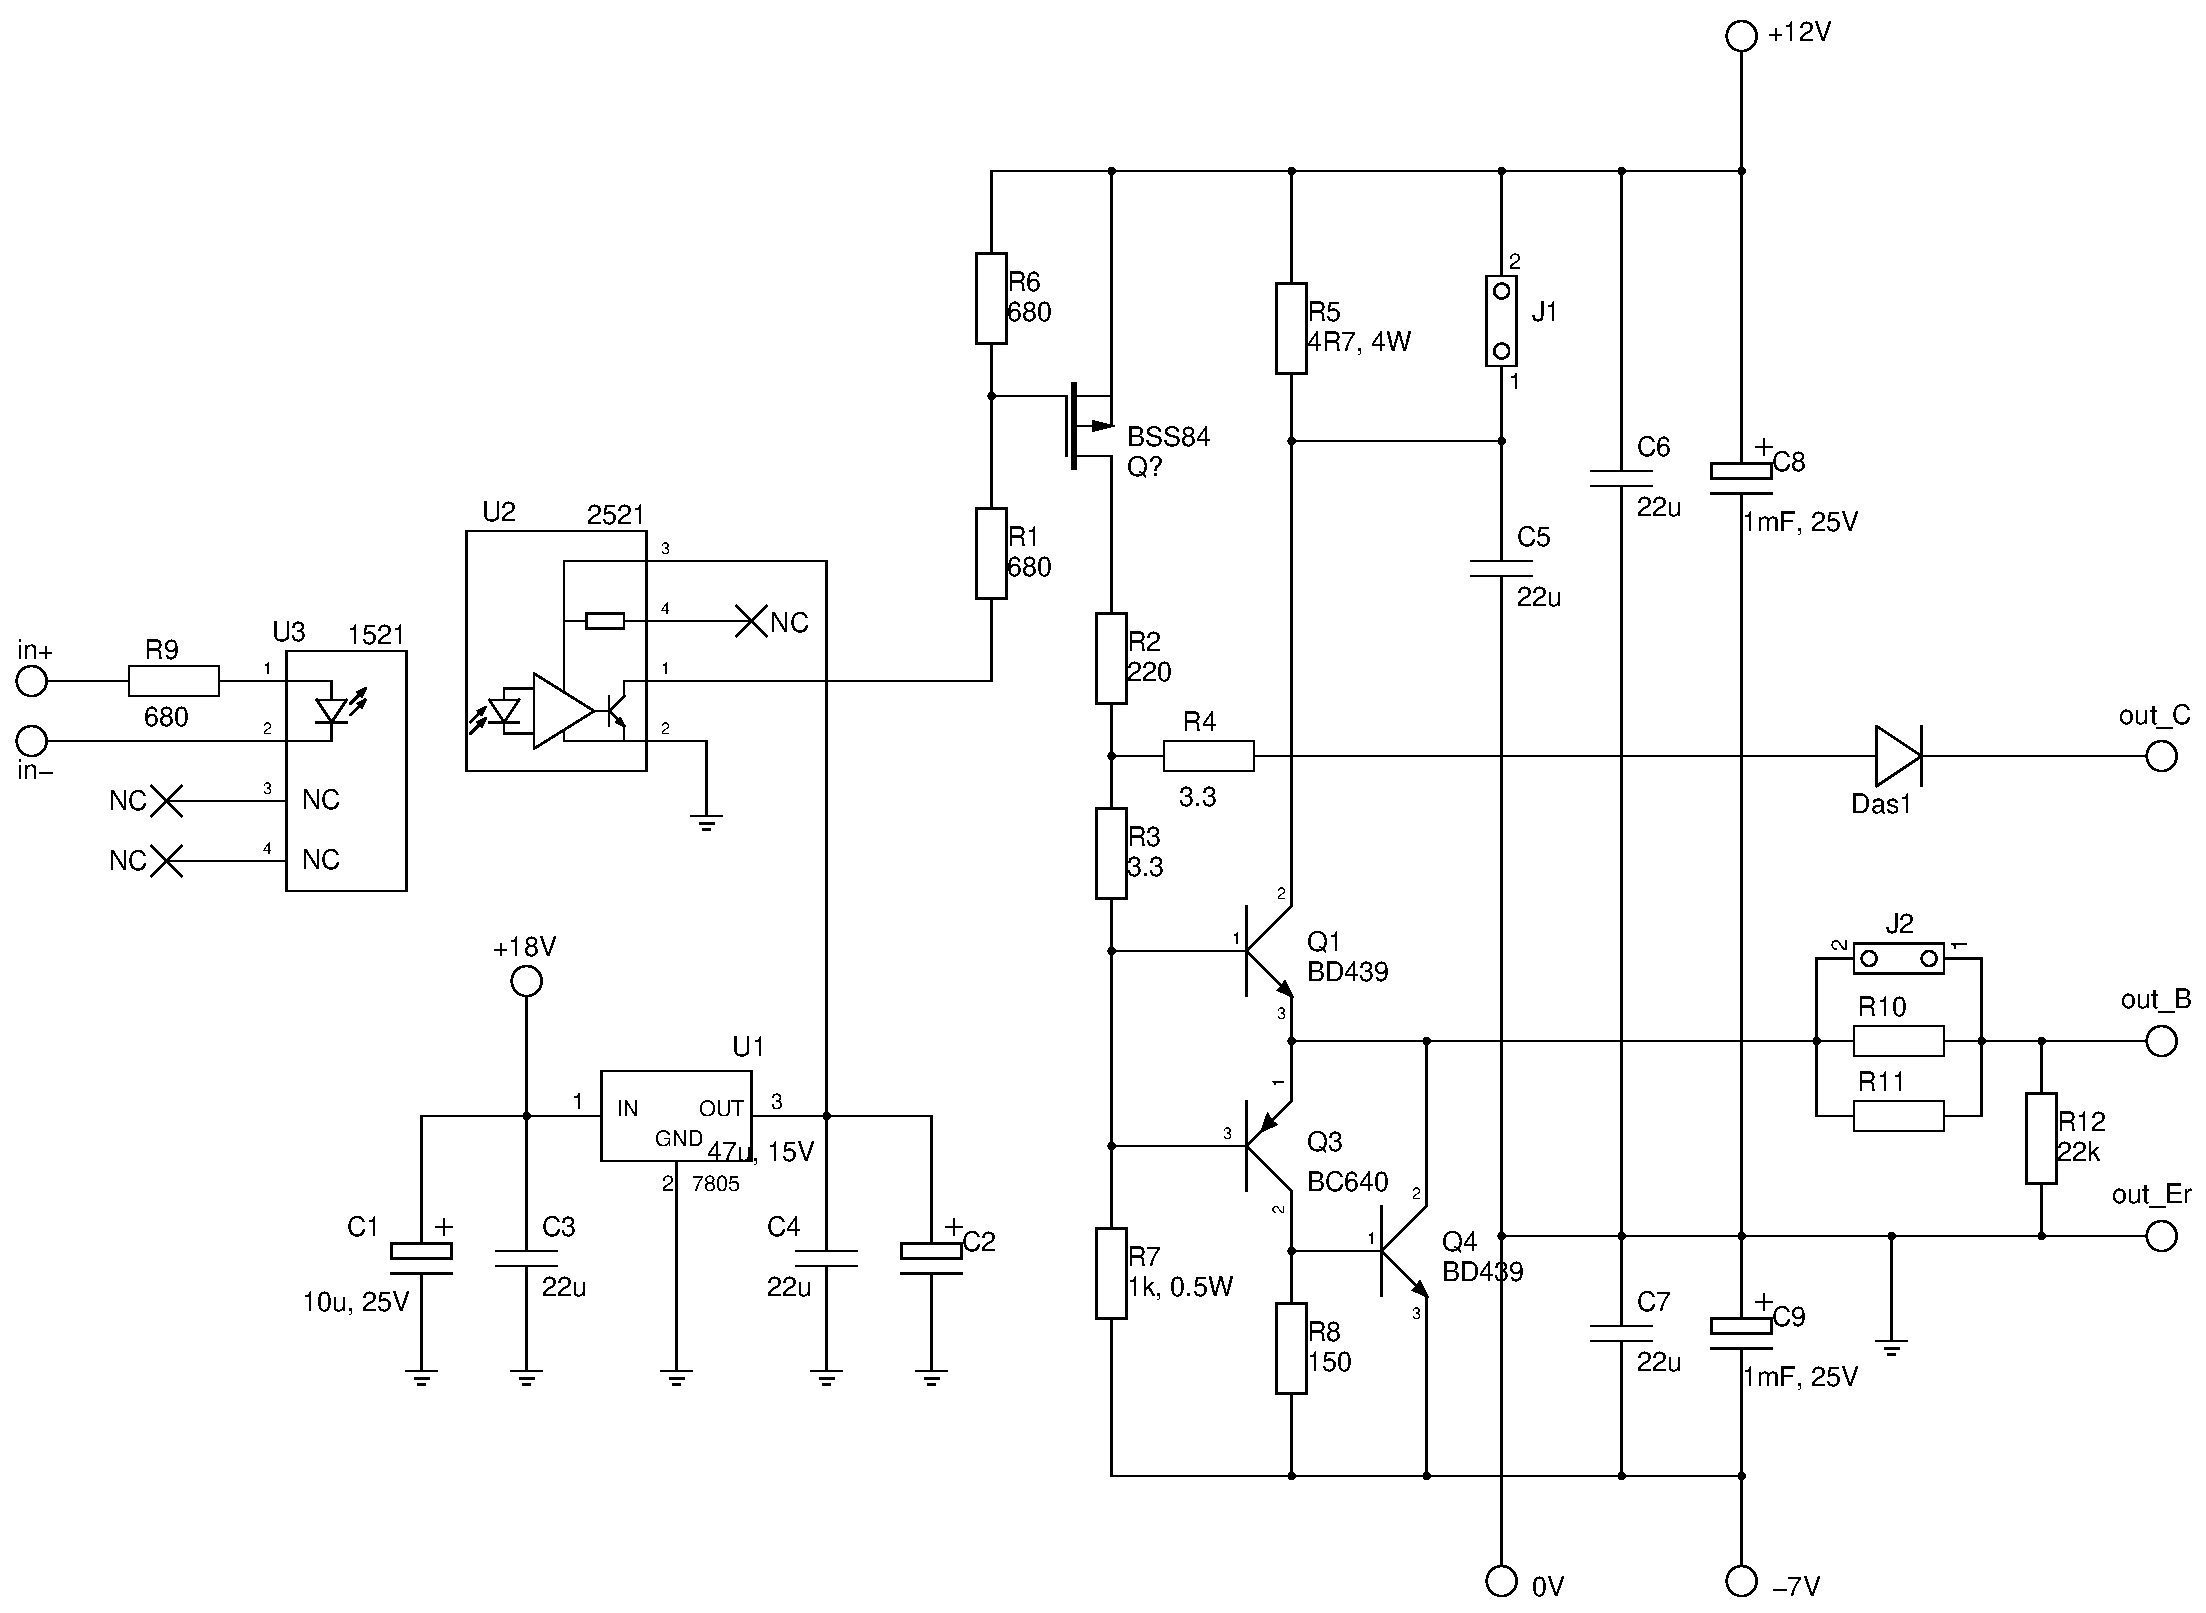
\includegraphics[width=1.2\textwidth]{schema_budic2}


\subsection{DPS}
DPS a rozmiestnenie súčiastok(1:1). Zľava: top assembly, bottom, bottom assembly:\vspace{0pt}

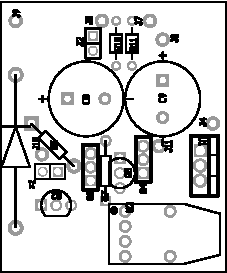
\includegraphics{pcb_budic_top_ass}
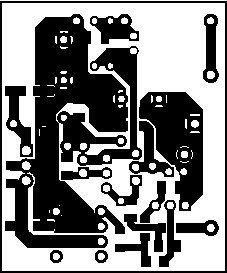
\includegraphics{pcb_budic_bot}
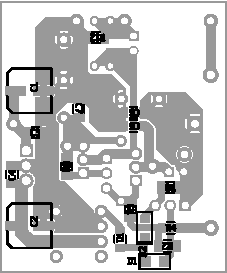
\includegraphics{pcb_budic_bot_ass}

\newpage
\subsection{Zoznam súčiastok}
\small
\begin{verbatim}

refdes   device                    footprint                     value    

C1       POLARIZED_CAPACITOR       NICHICON_WT_CAP_6p3_7p7       10u/25V
C2       POLARIZED_CAPACITOR       NICHICON_WT_CAP_6p3_7p7       47u/15V
C3       CAPACITOR                 1206.fp                       22u
C4       CAPACITOR                 1206.fp                       22u
C5       CAPACITOR                 1206.fp                       22u
C6       CAPACITOR                 1206.fp                       22u
C7       CAPACITOR                 1206.fp                       22u
C8       POLARIZED_CAPACITOR       RCY250P                       1mF/25V
C9       POLARIZED_CAPACITOR       RCY250P                       1mF/25V
D1       DIODE                     minimelf                      1N4148
D2       DIODE                     minimelf                      1N4148
Das1     DIODE                     DIODE_LAY 800.fp              [1000V]
J1       JUMPER                    JUMPER2.fp                             
J2       JUMPER                    JUMPER2.fp                             
Q1       NPN_TRANSISTOR            TO126W.fp                     BD439    
Q2       PNP_TRANSISTOR            TO92.fp                       BC640    
Q3       PNP_TRANSISTOR            TO92.fp                       BC640    
Q4       NPN_TRANSISTOR            TO126W.fp                     BD439    
R1       RESISTOR                  1206.fp                       3k3      
R2       RESISTOR                  1206.fp                       220      
R3       RESISTOR                  1206.fp                       33       
R4       RESISTOR                  1206.fp                       33       
R5       RESISTOR                  ACY400                        "4R7/4W"          
R6       RESISTOR                  1206.fp                       1k       
R7       RESISTOR                  ACY300                        "2k2/0.5W"        
R8       RESISTOR                  1206.fp                       150
R9       RESISTOR                                                680
R10      RESISTOR                  0.125W_Carbon_Resistor                 
R11      RESISTOR                  0.125W_Carbon_Resistor                 
R12      RESISTOR                  1206.fp                       22k      
U1       7805                      TO220W.fp                              
U2       fiber_optic_receiver                                    2521     
U3       fiber_optic_transmitter                                 1521     
\end{verbatim}
\normalsize
\newpage
\section{Napájací obvod budiča} \label{sec:append_nap}
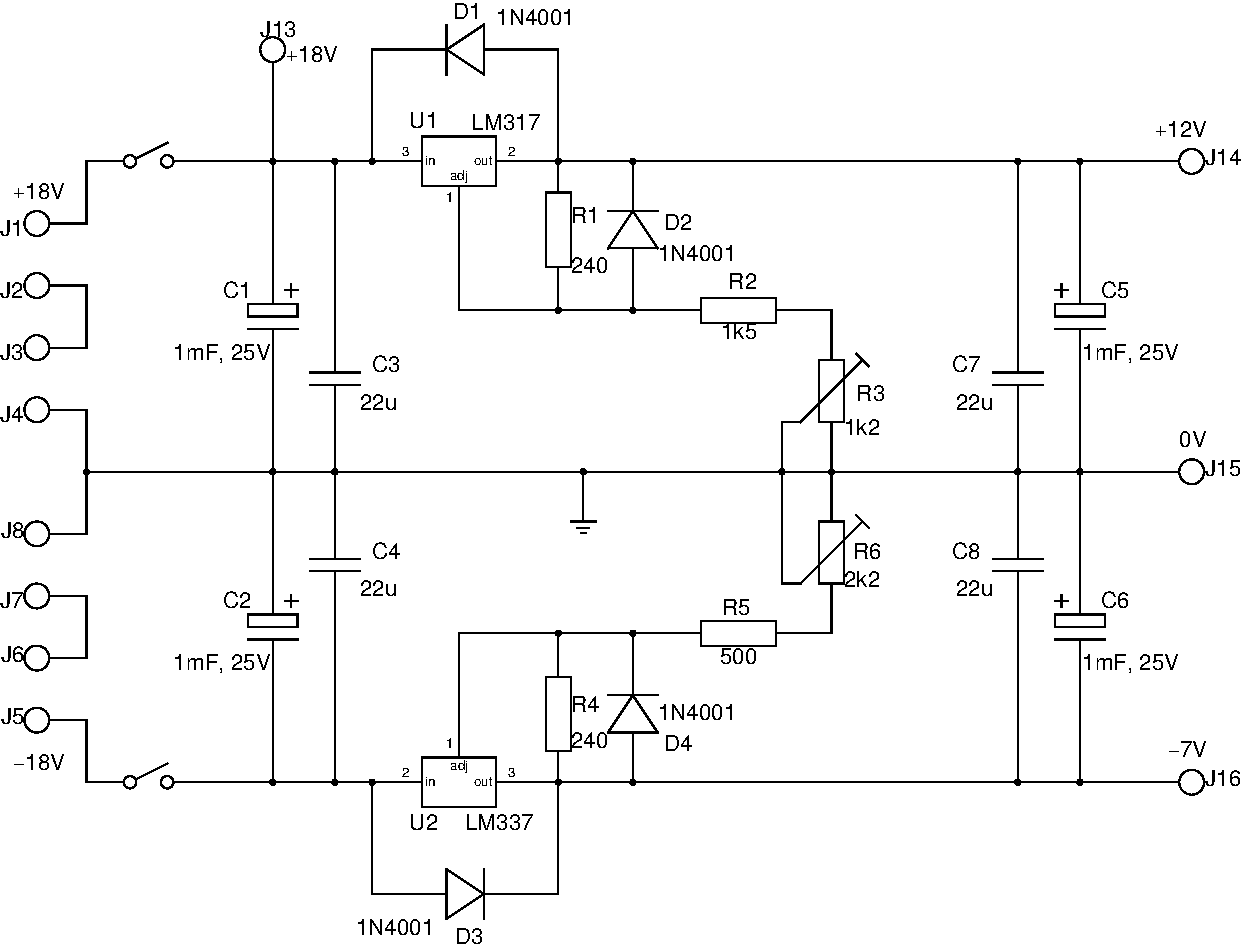
\includegraphics[width=.8\textwidth]{schema_nap}

\subsection{DPS}
DPS a rozmiestnenie súčiastok. Zľava: top assembly, bottom, bottom assembly:\vspace{5pt}

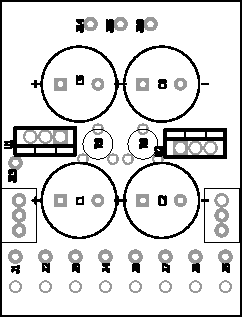
\includegraphics{pcb_nap_top_ass}
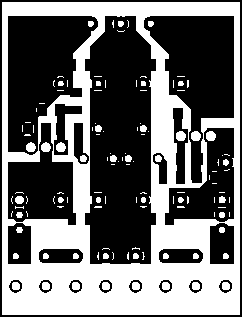
\includegraphics{pcb_nap_bot}
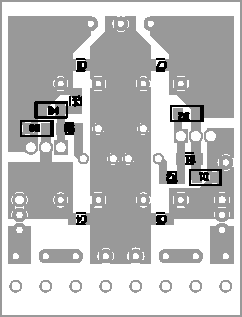
\includegraphics{pcb_nap_bot_ass}

\newpage
\subsection{Zoznam súčiastok}
\small
\hspace{2cm}
\begin{verbatim}
refdes   device                         footprint            value    

C1       POLARIZED_CAPACITOR            RCY250P              1mF/25V
C2       POLARIZED_CAPACITOR            RCY250P              1mF/25V
C3       CAPACITOR                      1206                 22u      
C4       CAPACITOR                      1206                 22u      
C5       POLARIZED_CAPACITOR            RCY250P              1mF/25V
C6       POLARIZED_CAPACITOR            RCY250P              1mF/25V
C7       CAPACITOR                      1206                 22u      
C8       CAPACITOR                      1206                 22u      
D1       DIODE                          melf                 1N4007   
D2       DIODE                          melf                 1N4007   
D3       DIODE                          melf                 1N4007   
D4       DIODE                          melf                 1N4007   
R1       RESISTOR                       1206                 240      
R2       RESISTOR                       1206                 1k5      
R3       VARIABLE_RESISTOR              trimmer_lezaty_5mm   1k2      
R4       RESISTOR                       1206                 240      
R5       RESISTOR                       1206                 500      
R6       VARIABLE_RESISTOR              trimmer_lezaty_5mm   2k2      
U1       adjustable_voltage_regulator   TO220W               LM317    
U2       adjustable_voltage_regulator   TO220W               LM337    
\end{verbatim}
\normalsize




\newpage
\section{Generátor impulzov} \label{sec:append_gen}

\subsection{Schéma zapojenia}
\hspace{-1.0cm}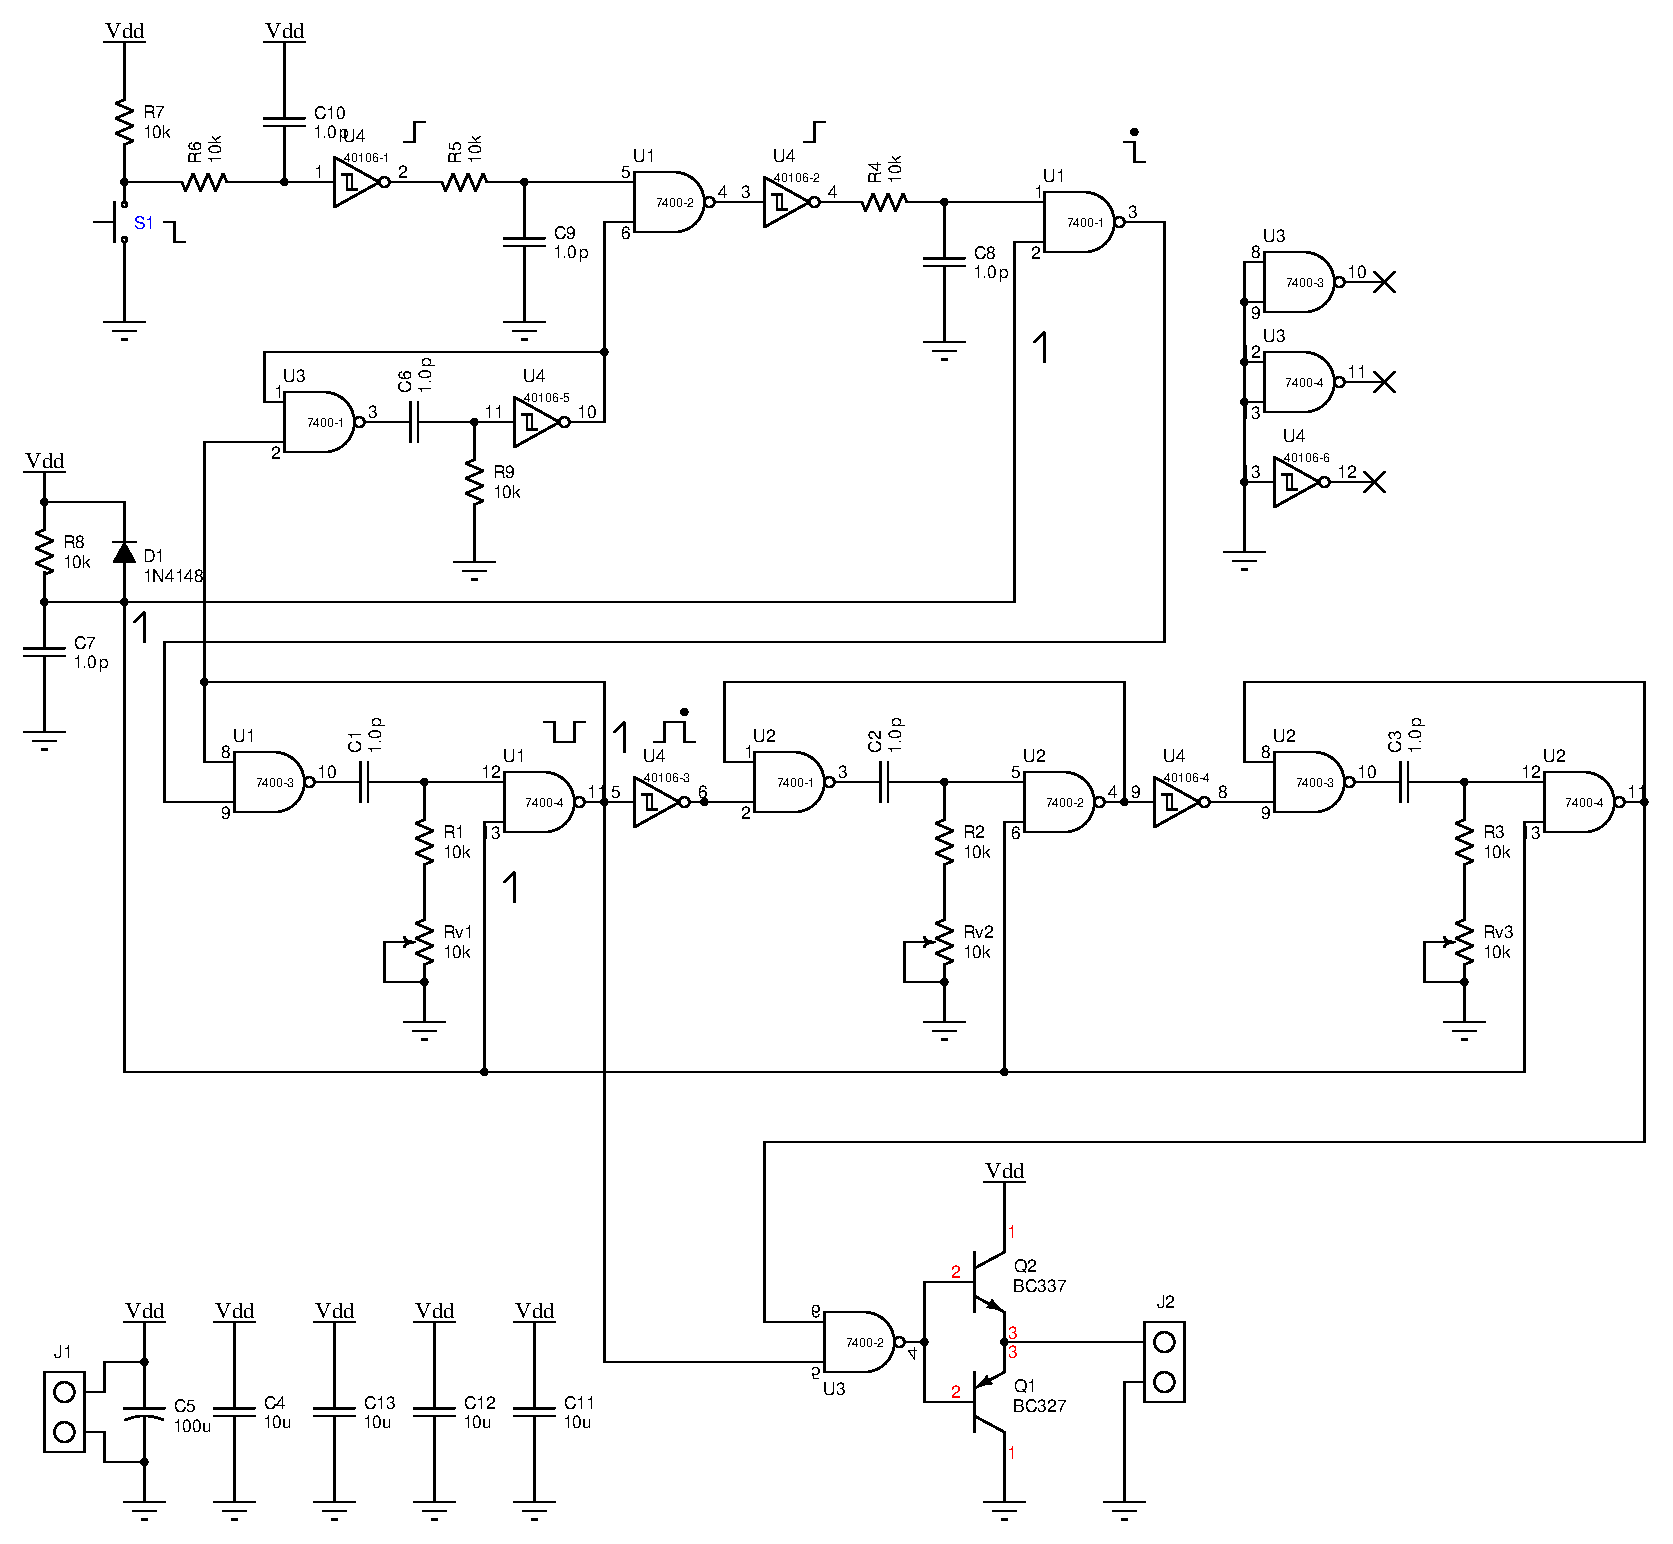
\includegraphics[width=1.25\textwidth]{schema_gen}

\newpage
\subsection{DPS}
DPS a rozmiestnenie súčiastok (1:1). Zľava: top assembly, bottom:\vspace{5pt}

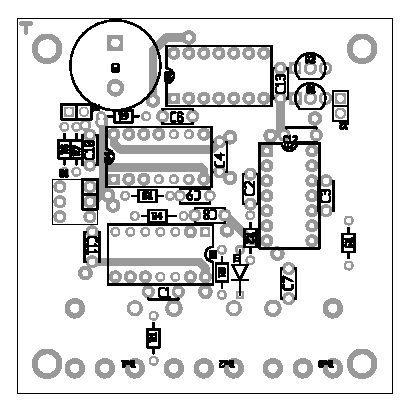
\includegraphics{pcb_gen_top_ass}

\includegraphics{pcb_gen_bot}

%\newpage
%\subsection{Zoznam súčiastok}
%\small
%\hspace{2cm}
%\begin{verbatim}
%\end{verbatim}
\normalsize



\newpage
\section{Medziobvod} \label{sec:append_medziobvod}

\subsection{Schéma zapojenia}
\vspace{10pt}
\hspace{-1.0cm}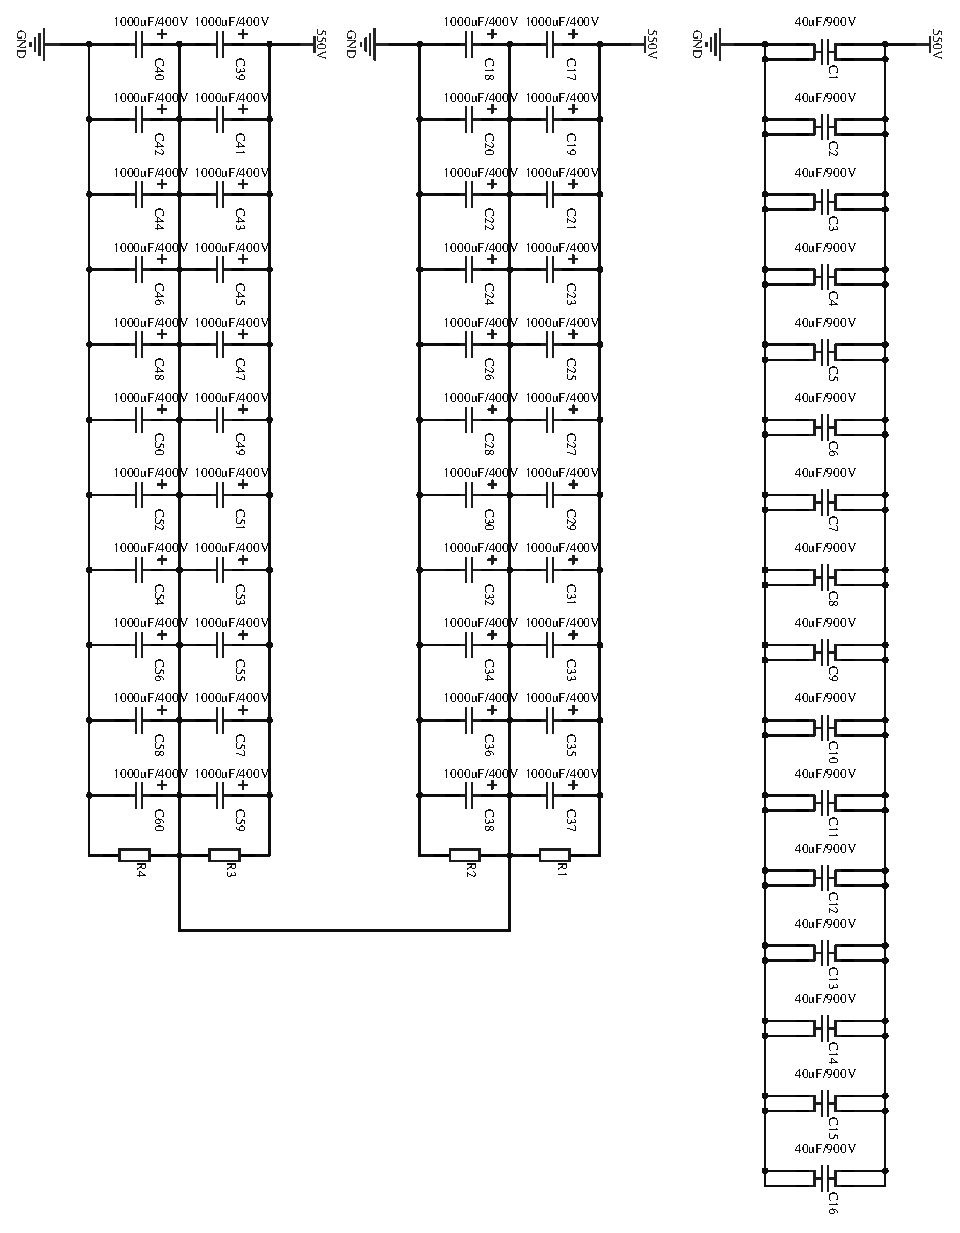
\includegraphics[width=1.1\textwidth]{schema_medziobvod_90}

\newpage
\subsection{DPS}
DPS a rozmiestnenie súčiastok (zmenšené). V poradí: top, bottom, bottom assembly:\vspace{5pt}
\centering
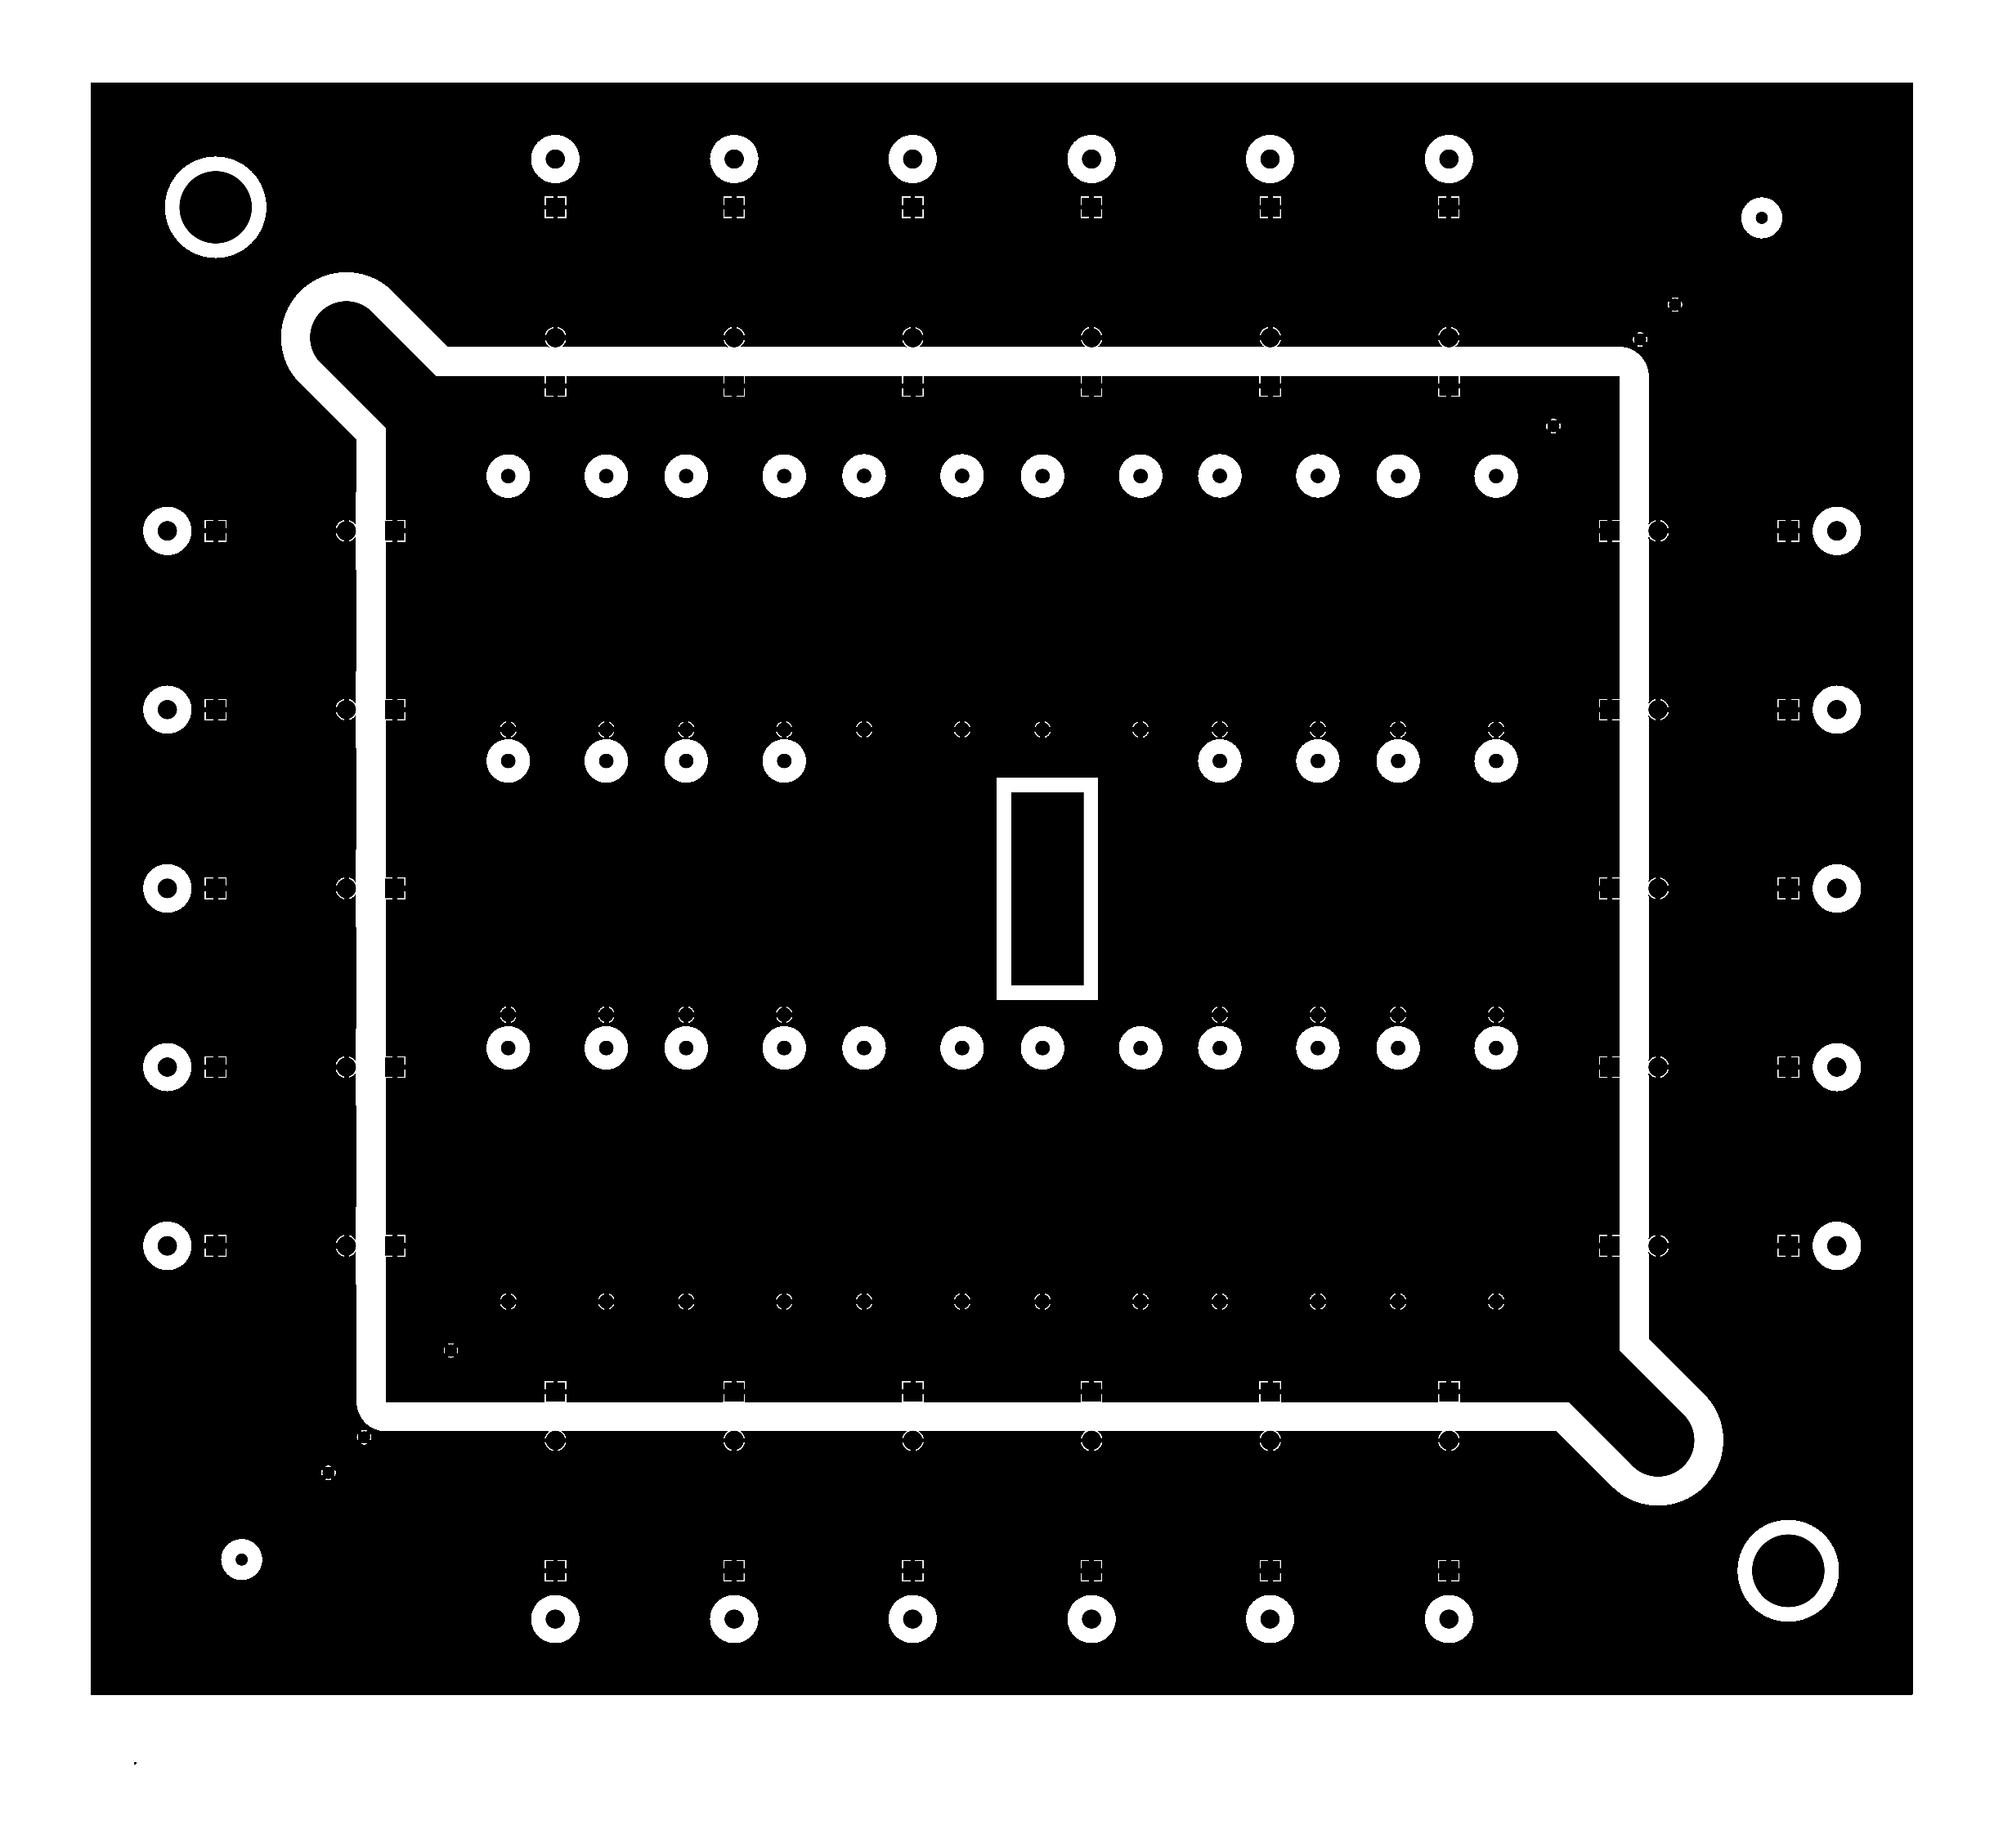
\includegraphics[width=\textwidth]{pcb_medziobvod_top}
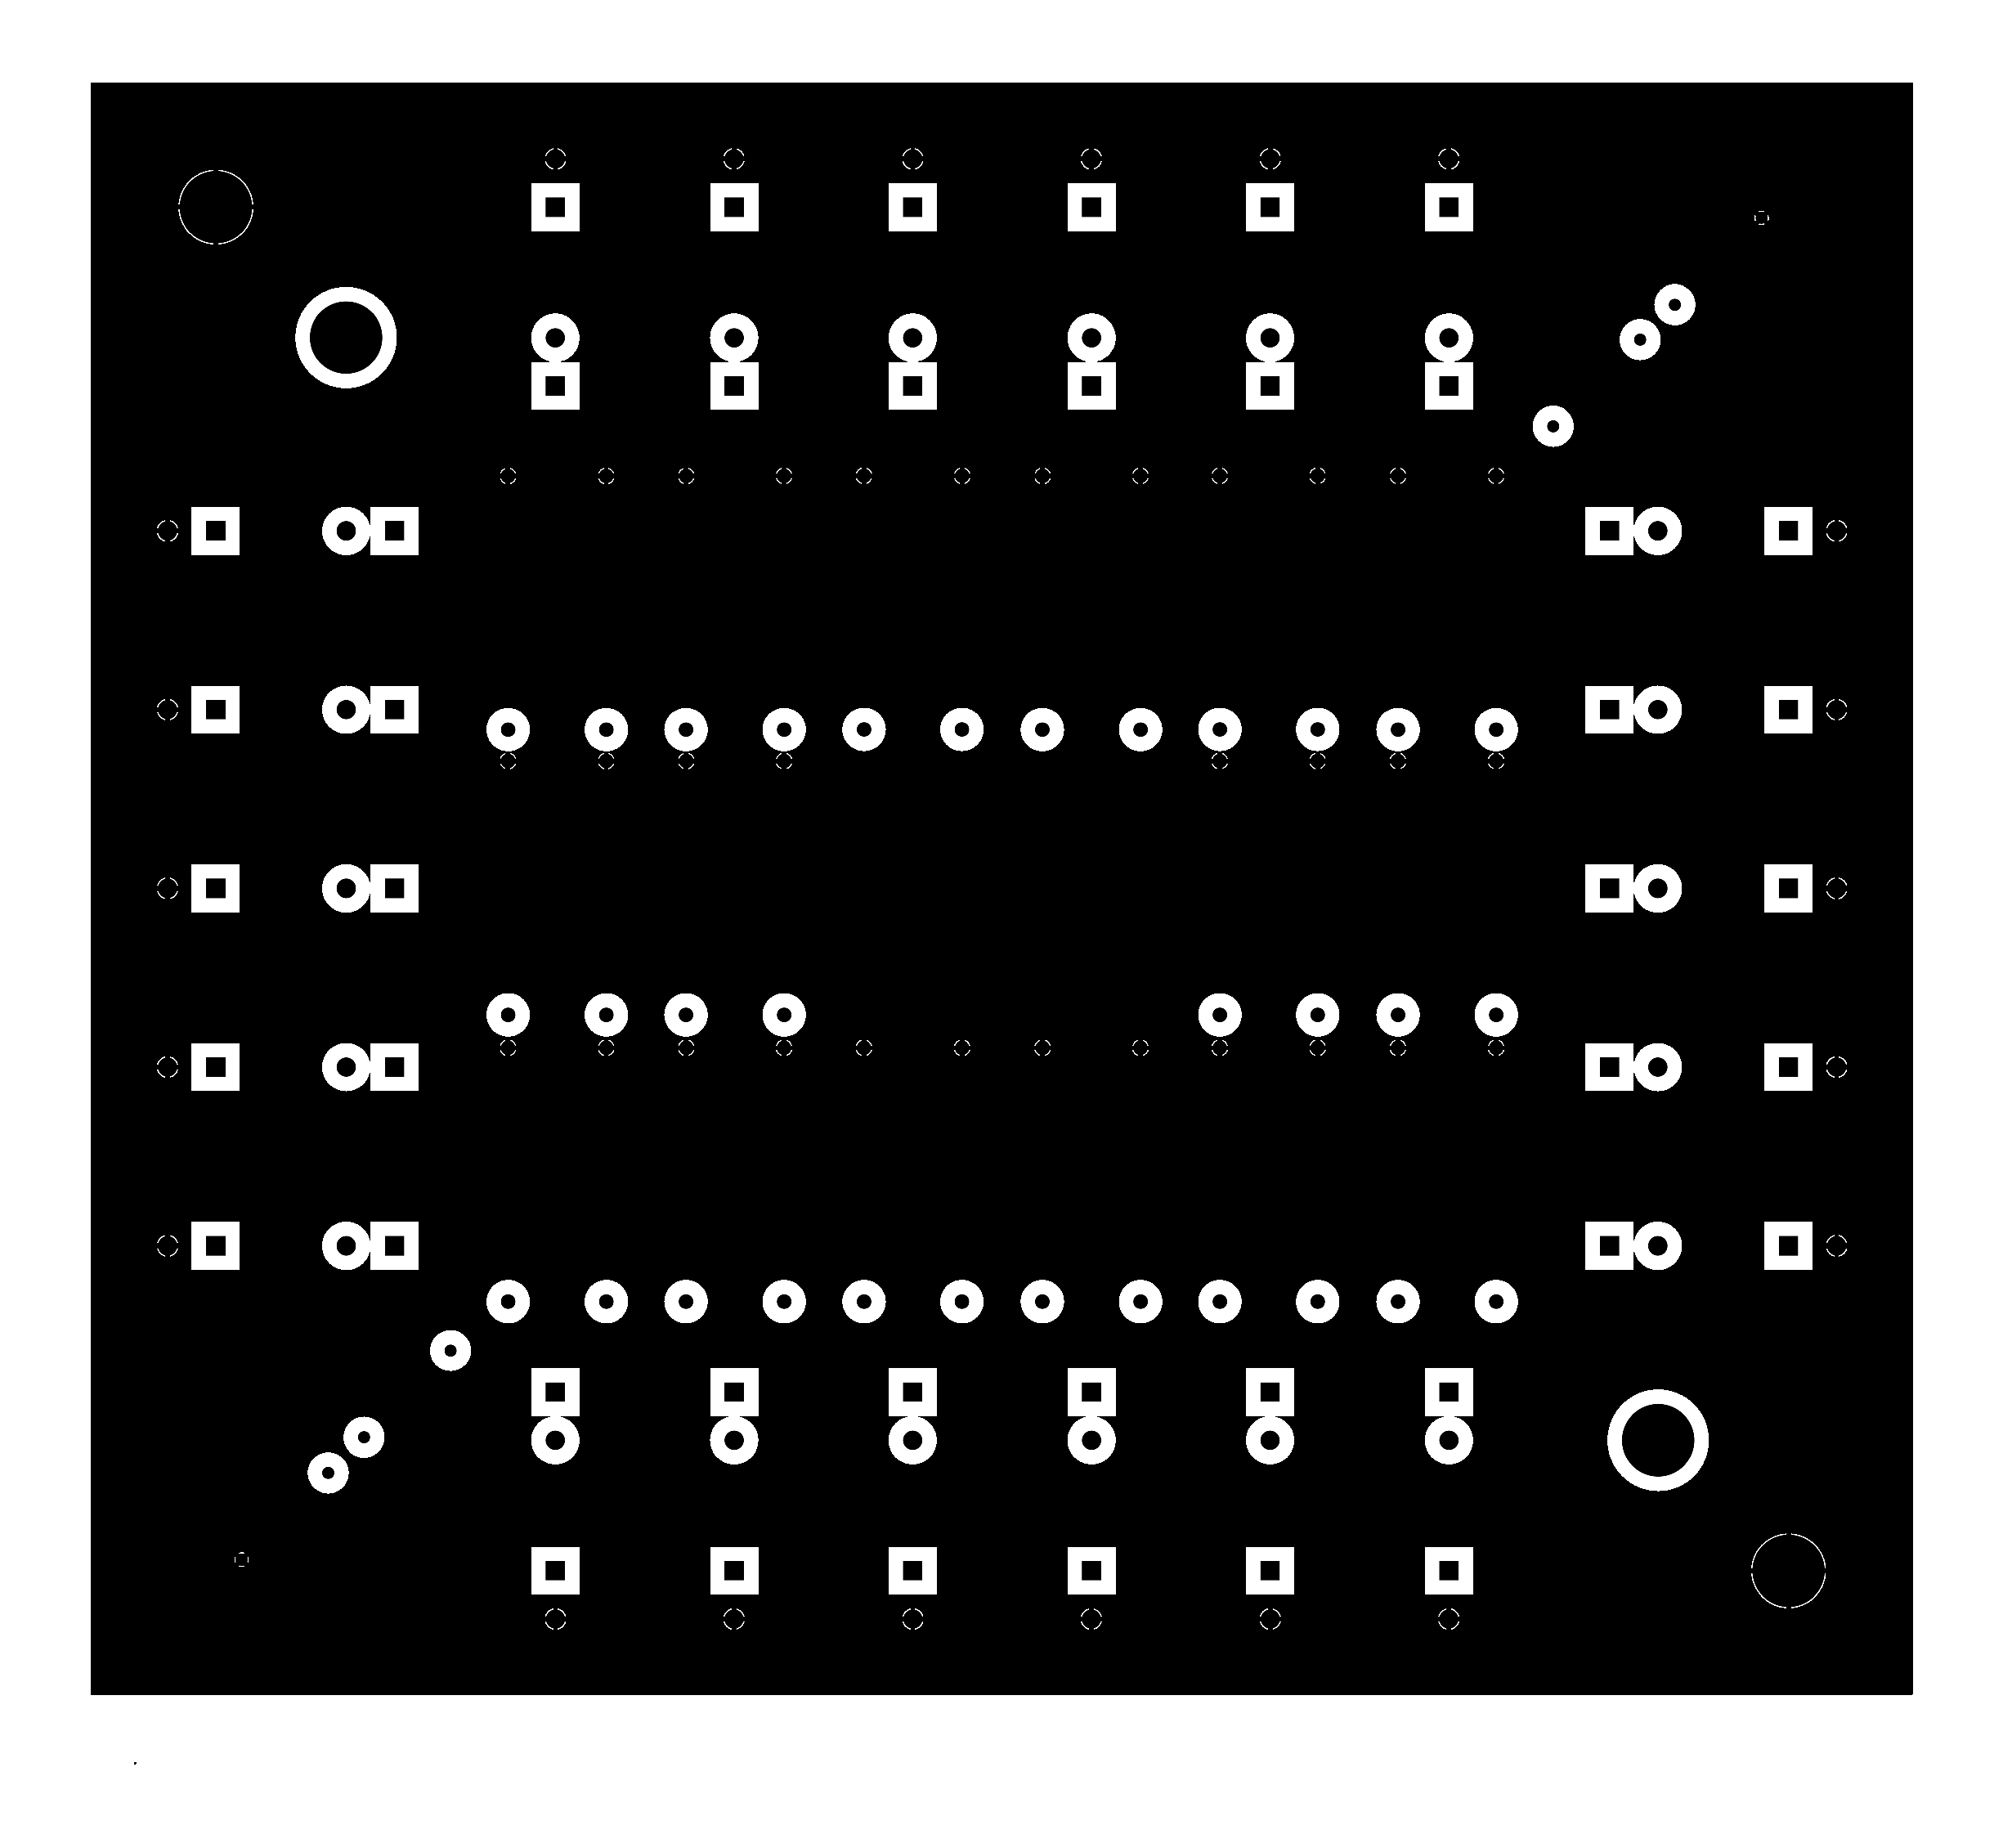
\includegraphics[width=\textwidth]{pcb_medziobvod_bot}
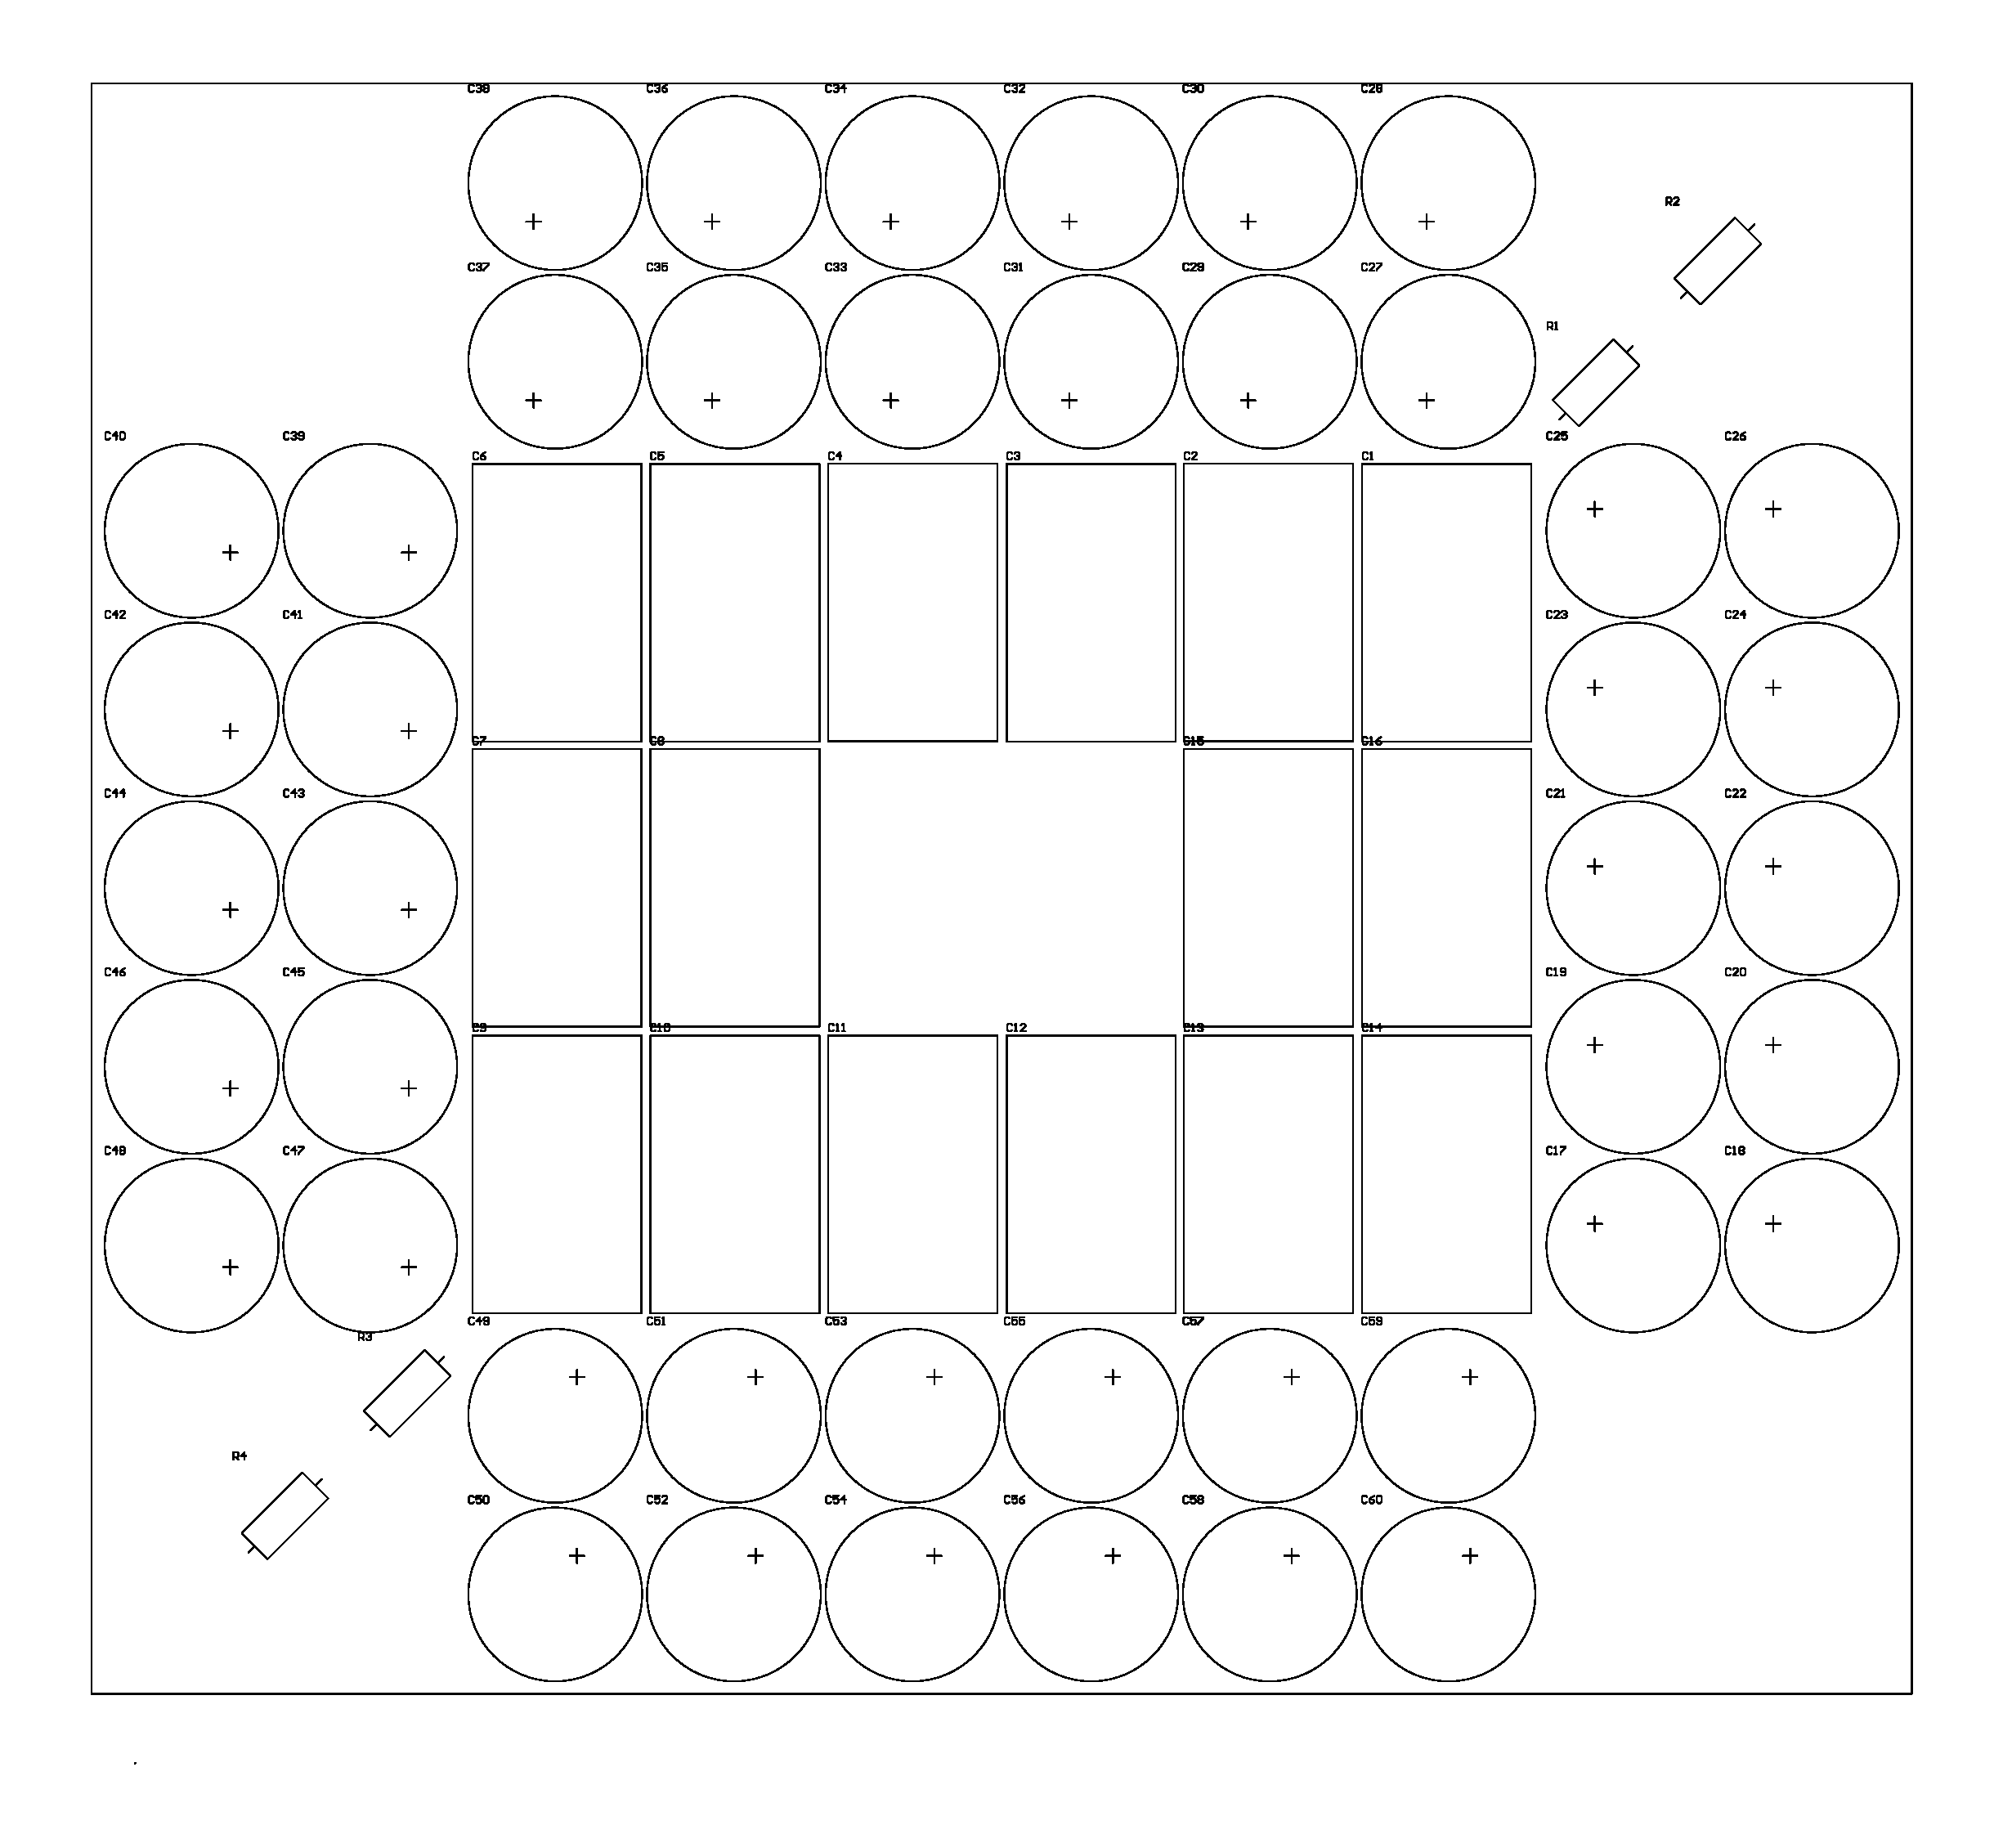
\includegraphics[width=\textwidth]{pcb_medziobvod_bot_ass}

%\newpage
%\subsection{Zoznam súčiastok}
%\small
%\hspace{2cm}
%\begin{verbatim}
%\end{verbatim}
\normalsize



\label{LastPage}
\end{document}
